
%使用XeLaTeX编译
%版权所有,翻版必究
%本文件由程序自动生成,任何修改将被覆盖
%2019 年 01 月 23 日




%\FloatBarrier
\cleardoublepage
\chapter{
从C{\sourcefonttwo{}+}{\sourcefonttwo{}+}扩展Qt Quick
}\label{c000012}


%begin图片
\begin{figure}[htb] %浮动体 here and top ...
%there must use marginnote ...
\marginnote{\setlength\fboxsep{2pt}\fbox{\footnotesize{\kaishu\figurename\,}\footnotesize{\ref{p000070}}}}\centering %中心对齐
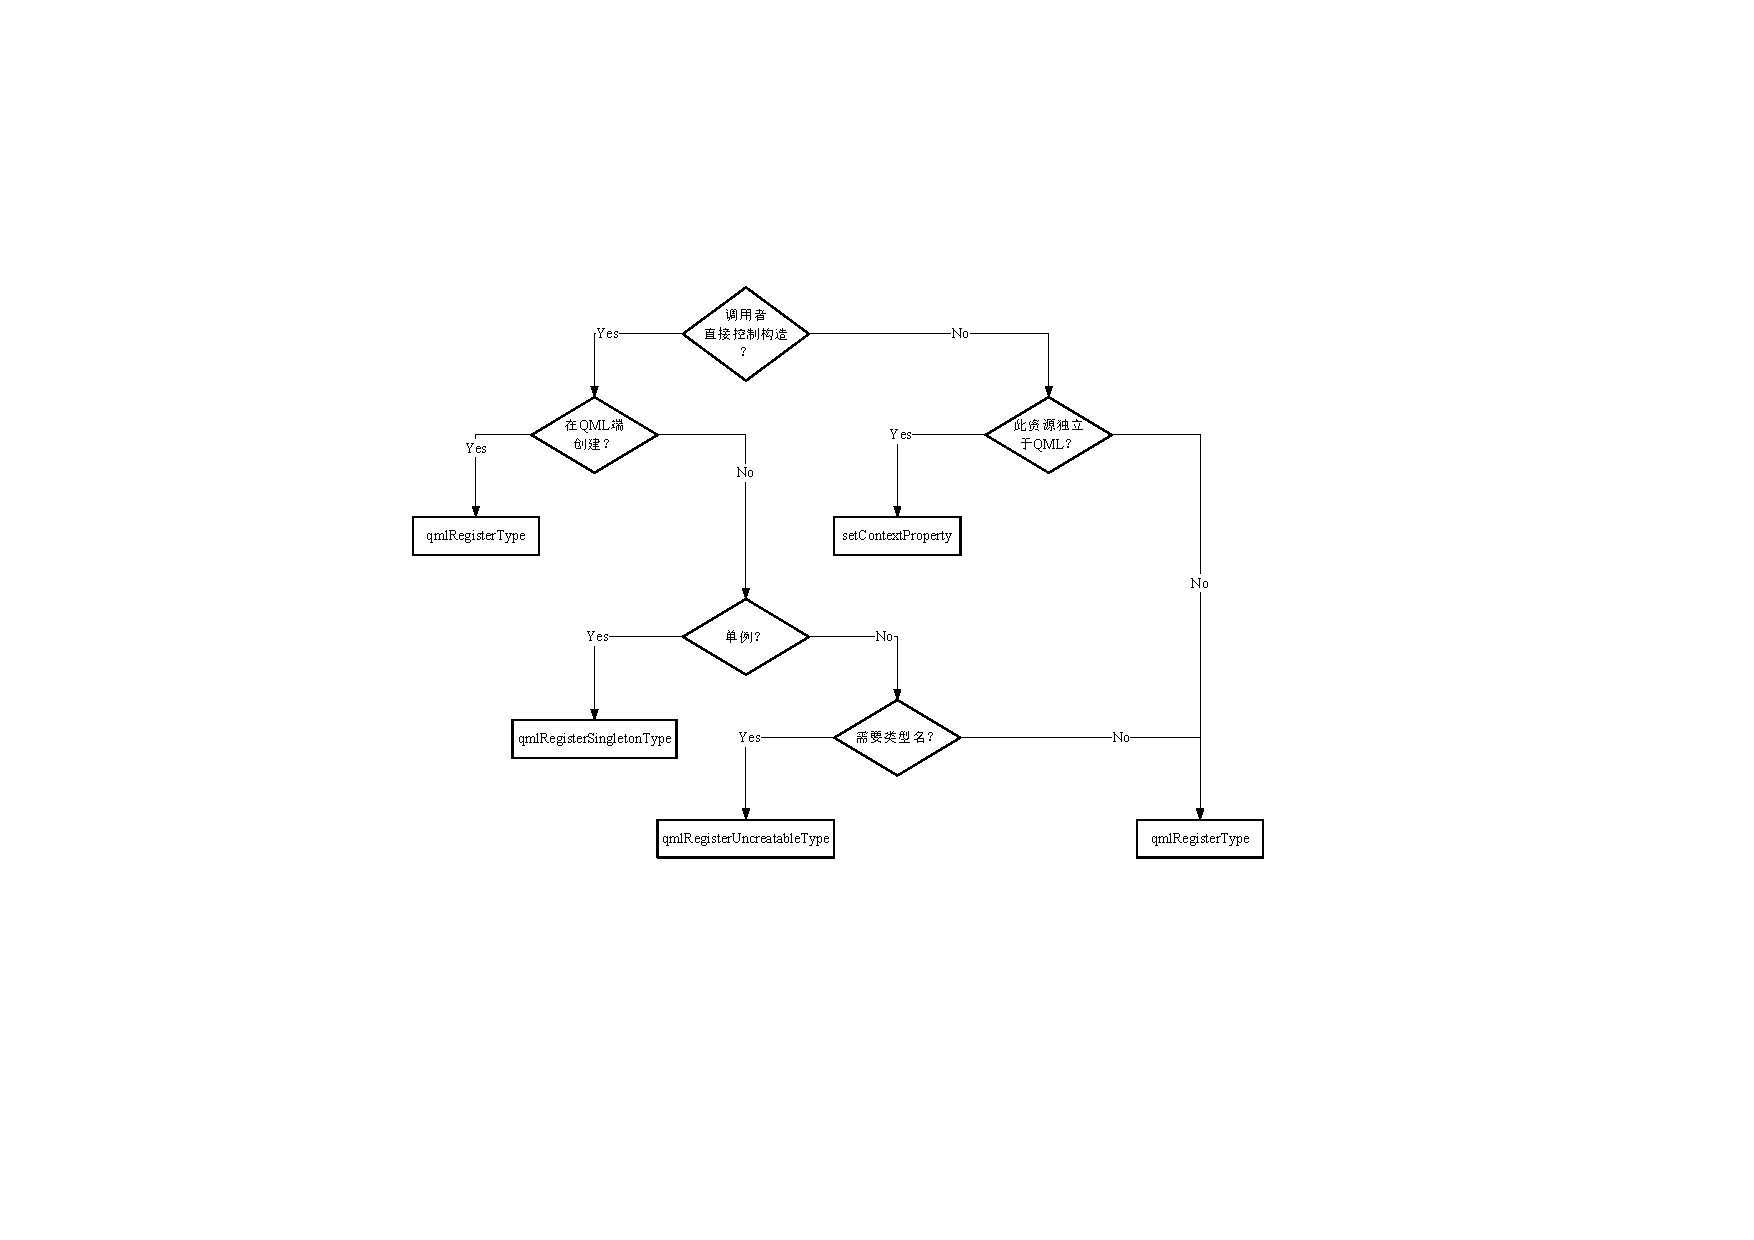
\includegraphics[width=0.95\textwidth]{chapter03/images/ChoosingTheCorrectIntegrationMethodBetweenCppAndQML.pdf} %图片路径
\caption{bigscene} %标题
\label{p000070} %索引
\end{figure}
%end图片



% ______all_key_words
% the_book_chapter the_book_subsection the_book_subsubsection
% the_book_section the_book_image the_book_table
% the_book_file the_book_tree_file the_book_command_file
% littlelongworld tabbing ref
% figurename tablename filesourcenumbernameone
% treeindexnumbernameone commandnumbernameone footnote
% item itemize comment textbullet
% \hspace*{\parindent}
% FloatBarrier







%使用XeLaTeX编译
%版权所有,翻版必究
%本文件由程序自动生成,任何修改将被覆盖
%2019 年 01 月 23 日



